\documentclass[conference]{biblio/IEEEtran}
\IEEEoverridecommandlockouts
% The preceding line is only needed to identify funding in the first footnote. If that is unneeded, please comment it out.
\usepackage[numbers]{natbib}
\usepackage{amsmath,amssymb,amsfonts}
\usepackage{graphicx}
\usepackage{textcomp}
\usepackage{xcolor}
\usepackage{hyperref}
\def\BibTeX{{%! suppress = PrimitiveStyle
\rm B\kern-.05em{%! suppress = PrimitiveStyle
\sc i\kern-.025em b}\kern-.08em
T\kern-.1667em\lower.7ex\hbox{E}\kern-.125emX}}

\begin{document}

\title{How smart grid testing can benefit from cloud testing - A literature review\\}

\author{\IEEEauthorblockN{Wildermuth Salome}
\IEEEauthorblockA{\textit{Department of Informatics} \\
\textit{University of Zurich}\\
Zurich, Switzerland \\
salome.wildermuth@uzh.ch}}


\maketitle


\begin{IEEEkeywords}
Smart grid, IoT, Cloud testing, Cloud computing
\end{IEEEkeywords}

\begin{abstract}
The present document contains a review on the topic of cloud testing approaches that have been applied in the domain of smart grid testing so far. Intelligent electrical supply systems are subject to an emerging field of research, especially the related risks of cyber security attacks and the challenge of processing high data volumes in real-time. The review emphasizes scientific papers from 2018 - 2023 about penetration and performance testing of cloud-based IoT devices, like smart meters, and metering infrastructure, like communication networks or data management systems. (https://www.blackridgeresearch.com/blog/what-is-a-smart-grid-what-are-the-major-smart-grid-technologies))
\end{abstract}
 % Abstract and Zusammenfassung
\section{Introduction}
Being a substantial part of smart cities, evolving all around the globe, smart grids have gained increased focus from the society during the last years. Smart grids are electrical grids that replace manual by automated, i.e. digital / software-based monitoring, controlling and steering mechanisms of electrical flaws and electricity consumption. While smart grids open doors to unprecedented possibilities, like many other technological achievements, they have some downsides at the same time. Being part of the highly critical infrastructure of electricity supply, they are exceptionally exposed and vulnerable towards malicious attacks. Furthermore they face high-performance requirements in order to fulfill real-time data processing. Successful cyber attacks or misbehavior due to badly performing systems can cause huge damage to institutions and humans depending on this infrastructure.

Appropriate security and protection mechanisms and well designed software and hardware are inevitable to minimize these risks. Such systems require a high amount of thorough testing, especially with high focus to their vulnerabilities. Penetration and performance testing can be key to addressing the two main weaknesses of smart grids and cloud testing can make extended testing feasible by providing highly scalable test environments and resources.

This present review study emphasizes scientific papers from the years 2018 - 2023 containing research about penetration and performance testing of IoT devices, especially software for smart meters, communication networks and data management systems, in the cloud.

The search included manual document retrieval from four popular web libraries: IEEE, Google Scholar, Xplore and ACM Digital Library. From initially XX potential papers, XX were selected based on suitability criteria for the topic. Backward snowballing iterations have been done on the six most relevant papers, which added another XX papers to the review. The documents have been retrieved by using the following search terms in different combinations: smart grid, cloud testing, cloud computing, IoT, penetration testing, performance testing, testbed, co-simulation.

\section{Related Work}

Many authors investigated on IoT cloud computing and emphasize its potential to improve efficiency and reduce costs in IoT because computing resources can be scaled and virtualized in a flexible manner. \citeauthor{laghari2021review} in their \textit{Review and State of Art of Internet of Things} point out the tight interconnection between cloud and IoT and they emphasize advantages that the intermingling of IoT and cloud have. \citeauthor{almolhis2020security} attest the beneficial characteristics of cloud computing in IoT technologies in terms of on-demand self-service, resource pooling, broad network, measured service, and rapid elasticity. However, the large part of literature agrees repeatedly on criticalities of the cloud IoT, like security, data ownership, potential crashes and latency and \citeauthor{almolhis2020security} recommend to put immediate attention in the research community especially on open security topics.

\begin{figure}[htbp]
\centerline{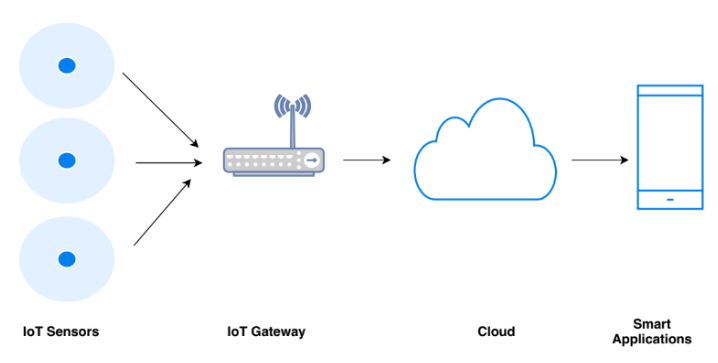
\includegraphics[scale=0.35]{images/iot_cloud_application_scenario.png}}
\caption{Sample of IoT cloud application scenario by \citeauthor{almolhis2020security}}
\label{fig}
\end{figure}

In the context of smart grids, the term \textit{hybrid-cloud usage} appears frequently and seems to be clearly favoured over "cloud-only" approaches for several reasons. \citeauthor{talaat2020hybrid} for example suggest to integrate data processing hardware devices to a private cloud to overcome security issues in the public cloud. \citeauthor{zahoor2018cloudmanag} recommend cloud-fog-based smart grid model for efficient resource management \cite{zahoor2018cloudmanag} and utilization \cite{zahoor2018cloudutil}. They explain how the amount of transmitted data and data transmission time can be significantly reduced because the fog approach reduces the amounts of data transmitted to the cloud by performing decentralized data processing. It means that some of the processing units and storage is placed closer to where data is actually being sourced from. It can furthermore address security issues and certain regulations (e.g. in relation to data ownership).

\citeauthor{7396147} investigate in how IoT systems' governance can be improved in terms of uncertainty in the system infrastructure. Uncertainty can be caused by many reasons, e.g. probe failures, network issues or human error and puts a lot of burden on the developers and operation mangagers (users) when managing runtime governance in IoT cloud systems \cite{7396147}. But it is a big challenge to include uncertainties in the development of proper governance strategies. \citeauthor{7396147} introduce the U-GovOps framework for \textit{dynamic, on-demand governance of elastic IoT cloud systems under uncertainty}. It consists of a declarative policy language that basically allows the developers to model uncertainties for their governance strategies and mechanisms that support the execution of the strategies taking the modeled uncertainties into account.

\citeauthor{bornhoft2013simulation} showed with a simulation model of a smart grid integration into an office building how much energy costs could be saved if the energy consumption was steered by taking a hypothetical dynamic price model into account. Depending on the current supply and demand of electricity, they reduced consumption or increased the amount energy stored in thermal energy storages. In their model, they could economize up to 31\% of their usual energy costs by optimizing the energy consumption depending on the current price of electricity.

Zurich has a test area called \textit{Greencity}, where the electricity utility of Zurich (ewz) maintains a pilot project in form of an integral energy infrastructure with intelligent power regulation mechanisms. \citeauthor{baumgartner2020monitoring} summarize findings about the \textit{monitoring concept suitable for utilising flexibilities in the low-voltage distribution grid in Greencity}. Their main focus was to gain experience with cloud architecture in terms of processing data collected by sensors. In the case of \textit{Greencity}, field data is streamed into a Microsoft Azure cloud computing environment for processing. They also seize on security and data protection issues in the context of using a cloud provider for hosting their services, but state that for their use case the Azure cloud architecture fulfils the information security requirements and for data protection they set up individual load profiles.

Testbeds represent a common experimentation platform where (prototypical) IoT devices or applications can be deployed and verified. According to \citeauthor{cintuglu2016cloud}, traditional testbeds tend to cover a limited project frame, while complex IoT systems, like smart grids, due to their interdisciplinary structure, require multiple heterogeneous test environments with different capabilities to interconnect in real-time. They therefore claim on more complete test platforms for comprehensive system testing and propose to include cloud communication for testbed implementation. They design a cloud-enabled architecture, where they outline the most relevant aspects how this can be achieved. Their proposal of a cloud enabled remote access smart grid testbed platform was implemented by the Energy Systems Research Laboratory, Florida International University.



\section{Research Methodology}
The research procedure consisted of three phases: review planning, conduction and reporting the results. This process was inspired by the recommendation of the guidelines in Kitchenham et. Al's \textit{Procedures for Performing Systematic Reviews} \cite{kitchenham2004procedures}. Even though this is not a \textit{systematic} review, the fundamental principle of the approach is still adequate and useful.

\subsection{Review planning}
The research question is about how cloud testing can be employed to test IoT systems like smart grids comprehensively. It gives an overview of the most important non-functional requirements, like cyber security, efficiency, reliability, and interoperability. It summarizes research findings about how cloud computing helps to solve but also aggravates some of these critical aspects.

To get a solid overview of the context, literature about vulnerabilities of smart grids and in general about risks posed in IoT development was examined. Smart grids are actually nothing else than a type of IoT ecosystem. They utilize sensors that collect data, streaming it on a central platform, which itself, processes and stores the data and implements APIs for devices and applications to enable interaction with the system. 

Next, it was investigated, if and how cloud replicas can help preventing system lacks in one of the above mentioned risk aspects. The section IV provides an overview of findings and discusses core statements regarding chances and difficulties as well as existing or proposed solutions.

\subsection{Review conduction}

The search for the literature review included manual document retrieval from three popular web libraries: IEEE eXplore, Google Scholar, and ACM Digital Library. The documents have been retrieved by using a search term combined of the keywords \textit{smart grid} or \textit{iot}, \textit {cloud}, and \textit{testing} or \textit{simulation}. The results were restricted to the years of publication from 2018 to 2023. The terms \textit{smart grid} and \textit{IoT} were treated as synonymous correspondants during the search and selection procedure, because it turned out that many findings for general IoT testing apply for smart grid testing. Equally, \textit{testing} and \textit{simulation} were treated according to the principle of synonymy. In the electrical engineering domain the term \textit{simulation} seems to be widespread and some papers use it more often than the term \textit{testing}.

From all documents retrieved by the search, those that met suitability criteria for the topic were selected in top down manner. Suitability was assessed in a two-step approach. Documents were directly selected, if they addressed all of the three above mentioned topics (\textit{smart grid} or \textit{iot}, \textit {cloud}, \textit{testing} or \textit{simulation}) in their title or abstract. If they covered at least two in title or abstract, they were pre-selected and then scanned for occurrences of the third missing keyword. For example the content of a document, with the title \textit{Cloud-Fog-based approach for Smart Grid monitoring} was scanned, if it also covered the term \textit{testing} or \textit{simulation} in the text. 

Finally, manual backward snowballing iterations have been done on research papers that cited other papers in relation to cloud testing solutions for smart grids or IoT  with publication date from 2018 to 2023.

\subsection{Terminology}
\citeauthor{bertolino2019systematic} conducted a \textit{systematic review on cloud testing} and they distinguish the term \textit{cloud testing} by two meanings: \textit{testing of the cloud (ToC)}, which refers to testing systems running in a cloud and \textit{testing in the cloud (TiC)} which refers to leveraging cloud technologies for testing. They find that the cloud \textit{offers the possibility to develop and maintain costly test infrastructures and to leverage on-demand scalable resources for configuration (by using cloud virtualization) and performance (by means of cloud elasticity) testing.} This literature review did not have a specific focus on one of the definitions. Both shapes of cloud testing were considered, as well as their intersection, which is called \textit{testing of the cloud in the cloud (ToiC)} by \citeauthor{bertolino2019systematic}.




\input{sections/sec4_review}
\section{Conclusion}

...



\bibliographystyle{biblio/IEEEtranN}
\bibliography{biblio/cloud-testing}

\vspace{12pt}


\end{document}
